In this project, we are following agile process development model as shown in figure \ref{fig:process_model} because this project requires adaptive planning along with evolutionary development and continuous improvement. The initial phase of the project is focused on gathering the software requirement.There will be two official milestones and several internal project team milestones, in order to deliver the product on time. Project deliverables are divided into sub-activities and for each activity a development cycle will be followed which will include different phases such as design, development, testing, review and improvement.
\paragraph{} Agile process development model (Shown on Fig.2) provides high customer satisfaction due to continuous delivery of the software modules and ensures the high quality software development. This model has advantages such as no planning is required to start the project as compared to other traditional software development models such as water fall in which project team makes strict promises to the client by doing requirement analysis and planning. This model is very easy to manage and provides great flexibility to the project team and client.

\paragraph{} For low level development and management, we used Scrum framework which is also a type of agile model. We decided to use this model because in this every one wants to get some experience in different phase of software development such as design, development , testing etc.

\begin{figure}
\centering
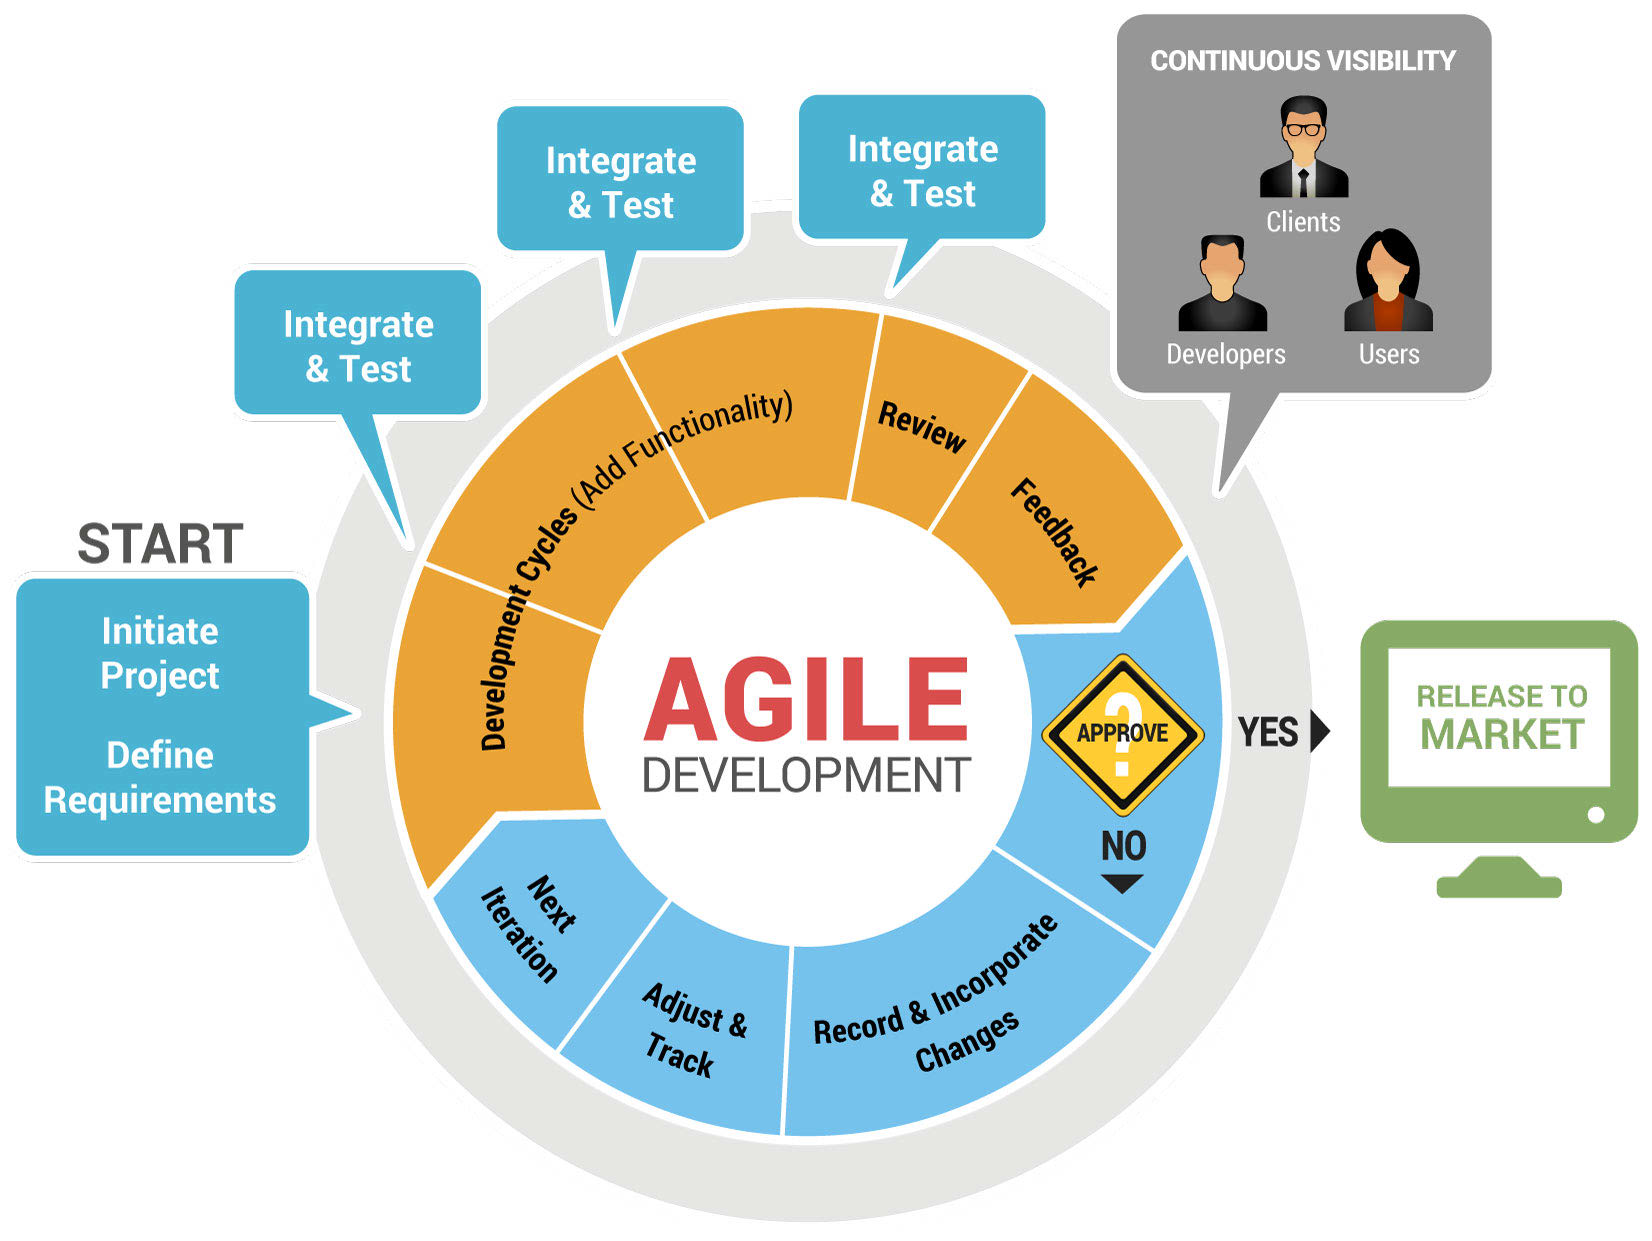
\includegraphics[width=0.9\textwidth]{process_model.png}
\caption{\label{fig:process_model}Agile process model diagram}
\end{figure}

